% Penn -> U.S. Dept. of Education / Default Resolution Group (FURNISHER direct dispute)
% SELF-CONTAINED: no \input, no external core file. Compile with XeLaTeX.
% Requires only the exhibit PDFs + signature.jpg in the same folder.
\documentclass[12pt,letterpaper]{article}
\usepackage[left=1.25in,right=1.25in,top=1in,bottom=1in]{geometry}
\usepackage{fontspec}
\usepackage{graphicx}
\usepackage{parskip}
\usepackage{enumitem}
\usepackage{titlesec}
\usepackage{booktabs}
\usepackage{array}
\usepackage{pdfpages}
\titleformat{\subsection}{\normalfont\bfseries}{\thesubsection}{1em}{}
\begin{document}

\begin{center}
  \textbf{VIA FACSIMILE AND CFPB PORTAL --- WRITTEN RECORD PRESERVED} \\
  \textbf{Date:} \underline{\today}
\end{center}

\begin{tabular}{@{}ll}
  \textbf{To:}   & U.S. Department of Education --- Federal Student Aid \\
                 & Attn: Richard Lucas, Chief Operating Officer, FSA \\
                 & and the Default Resolution Group \\
                 & P.O. Box 5609, Greenville, TX 75403-5609 \\
                 & \\
                 & \textit{cc:} Nicholas Kent, Under Secretary \\
                 & \hphantom{\textit{cc:} }Linda McMahon, Secretary \\
                 & \hphantom{\textit{cc:} }Office of the General Counsel \\
                 & \\
  \textbf{From:} & Ash Le' A. Penn \\
                 & 17548 NW Springville Rd \#9, Portland, OR 97229 \\
\end{tabular}
\vspace{1em}\hrule\vspace{1em}

\textbf{Borrower:} Ash Le' A. Penn (``Consumer''/``Borrower'') \\
\textbf{Social Security No.:} XXX-XX-7755 \quad \textbf{DOB:} 02/15/1988 \\
\textbf{Loan Program:} William D. Ford Federal Direct Loans \\

\begin{center}
  \textbf{Re: Formal Direct Dispute (FCRA \S~1681s-2(a)(8) / 12 C.F.R. \S~1022.43); \\
    Privacy Act Request to Amend (5 U.S.C. \S~552a(d)); \\
    Demand for Documentation}
\end{center}

\vspace{1em}
\textbf{Attached Exhibits:}
\begin{enumerate}[noitemsep]
  \item Valid State-Issued ID \& Current Utility Bill
  \item Equifax report 09/24/2024
  \item Equifax report 03/01/2026
  \item Master Promissory Note (¶20 highlighted)
  \item TransUnion Credit Report dated 03/01/2026 (showing expired removal dates)
  \item A copy of this dispute
\end{enumerate}
\vspace{1em}\hrule\vspace{1em}

To Whom It May Concern:

This is a formal direct dispute of the accuracy and completeness of the information the U.S. Department of Education, its servicer Nelnet, and its Default Resolution Group (collectively, ``the Department'') have furnished to the nationwide consumer reporting agencies regarding the Consumer's federal Direct Loans, submitted under FCRA \S~1681s-2(a)(8) and 12 C.F.R.\ \S~1022.43, as a Privacy Act request to amend agency records under 5 U.S.C.\ \S~552a(d), and as a demand for documentation. It is submitted in good faith and is not frivolous under 12 C.F.R.\ \S~1022.43(f). \textbf{Nothing herein is an admission or reaffirmation of any debt; the Consumer reserves all rights.}

\subsection*{The Reported Date of First Delinquency Is Self-Contradictory on Its Face}

The Department reports a Date of First Delinquency (DOFD) of \textbf{10/06/2024} (Default Resolution Group tradelines) and \textbf{11/05/2024} (Nelnet tradelines). That date cannot be reconciled with the reporting of these same accounts across the Consumer's own credit reports:

\begin{itemize}[noitemsep]
  \item The \textbf{Equifax report dated 09/24/2024} reports these accounts as current / paid as agreed, ``payment deferred,'' with the \textbf{Date of First Delinquency field blank}.
  \item The \textbf{TransUnion report} prints an estimated removal date of \textbf{08/2023} on these accounts --- a removal date that could only have been generated from a DOFD no later than 2016.
  \item The \textbf{Equifax report dated 03/01/2026} then reports a DOFD of \textbf{10/06--11/05/2024}.
\end{itemize}

\textbf{A single loan portfolio cannot simultaneously carry a blank date of first delinquency, a 2016-era date (implied by the 08/2023 removal date), and a 2024 date. These reportings are mutually exclusive and, on their face, establish that the date of first delinquency has been altered.} The burden is on the Department, and on the reinvestigating bureau, to substantiate the DOFD actually being reported --- not merely to confirm that it was ``verified.''

\subsection*{A Date of First Delinquency May Advance Only Upon a Substantiated Payment}

Under 15 U.S.C.\ \S~1681c(c)(1), the DOFD is fixed at the commencement of the delinquency that leads to the derogatory status and does not advance unless the account is brought current by an actual payment. If the Department contends that a payment reset or advanced the DOFD to 2024, \textbf{it must produce proof of that payment.} It has furnished none. To the contrary, the Department's own 09/24/2024 reporting shows these accounts with \emph{no date of first delinquency at all} --- confirming that, as of that date, no qualifying delinquency had been established, let alone one in 2024. Absent documented proof of a payment that advanced the date, the 2024 DOFD is unsubstantiated, and the seven-year reporting period --- which runs from the true DOFD and is a hard limit under 15 U.S.C.\ \S~1681c(a) --- renders these tradelines obsolete.

\subsection*{The Reported ``Date of Last Payment'' Is Unsupported and Irreconcilable}

The Department furnished a ``Date of Last Payment'' of \textbf{08/06/2023}. That entry cannot be reconciled with the Department's own contemporaneous reporting of these same accounts as ``over 120 days past due'' and never brought current, and --- on the 09/24/2024 report --- with no date of first delinquency. The Department must substantiate the 08/06/2023 entry with documented proof of an actual payment, or correct and delete it. A payment date that cannot be substantiated, used to support a later DOFD, is a willful accuracy violation under 15 U.S.C.\ \S~1681s-2(a)(1)(A).

\subsection*{Monthly Re-Publication}

Per the Equifax Data Furnisher Guidebook, a furnisher must report its full file (entire portfolio) each month. The Department therefore re-publishes the disputed DOFD every reporting cycle; each monthly furnishing is a separate, ongoing inaccuracy.

\subsection*{Structural Mismatch: Ten Collection Tradelines, Nine Loans}

Nine (9) originating Direct Loans appear on the Consumer's reports, yet \textbf{ten (10)} Default Resolution Group collection tradelines are being reported. One collection tradeline has no corresponding originating loan. A collection tradeline that does not map to an originating obligation cannot be verified and must be deleted.

\subsection*{Failure of the Required Pre-Reporting Notice}

Master Promissory Note Paragraph 20 provides: ``We will notify you at least 30 days in advance that we plan to report default information to a consumer reporting agency\ldots You will be given a chance to ask for a review of the debt before we report it.'' Independently, 15 U.S.C.\ \S~1681s-2(a)(7) requires written notice of negative information no later than 30 days after furnishing it, and the Debt Collection Act, 31 U.S.C.\ \S~3711(e), requires pre-report notice for federal debts.

The Department's own furnished data forecloses any claim that these obligations were met. On the 03/01/2026 report the Department furnished \textbf{Metro 2 Narrative Code 118 (``Customer Unable to Locate Consumer'')} on each tradeline:
\begin{itemize}[noitemsep]
  \item If Code 118 is accurate, the Department could not have provided the required notice, or the ¶20 review opportunity, before reporting.
  \item If Code 118 is inaccurate --- the Consumer's address, cellular number, and email were current and on file throughout the relevant period --- the Department furnished false information.
\end{itemize}
The Consumer does not concede inability to be located; the Department is held to its own certification. Under either reading, the adverse information cannot stand as furnished.

\subsection*{Demands}
\begin{enumerate}[label=\arabic*., leftmargin=*]
  \item Substantiate the Date of First Delinquency the Department is reporting (10/06--11/05/2024) by producing the complete account payment ledger and identifying the payment relied upon to advance it. Absent that substantiation, delete the tradelines as inaccurate and obsolete under \S~1681c(a).
  \item Substantiate the reported ``Date of Last Payment'' of 08/06/2023 with proof of an actual payment, or correct and delete it.
  \item Produce dated proof of the MPN ¶20 thirty-day advance notice and review opportunity, with proof of mailing/delivery, and of any \S~1681s-2(a)(7) notice.
  \item Reconcile the ten collection tradelines against the nine originating loans and delete any collection tradeline without a corresponding loan.
  \item Respond in writing within 30 days.
\end{enumerate}

\subsection*{Reservation of Rights}
Nothing herein waives any right or remedy, including FCRA \S\S~1681n and 1681o (willful and negligent noncompliance), which apply to the Department as a federal agency per \emph{Dept.\ of Agriculture Rural Development Rural Housing Service v.\ Kirtz}, 601 U.S.\ 42 (2024); FCRA \S~1681h(e); FCRA \S~1681i and \S~1681s-2(b) via the Consumer's parallel disputes to the bureaus; the Higher Education Act; the Privacy Act, 5 U.S.C.\ \S~552a; and the Debt Collection Act, 31 U.S.C.\ \S~3711.

\vspace{1.5em}\noindent Respectfully, \\ \vspace{1em}
\noindent 
\includegraphics[width=2.5in]{signature.jpg} \\
\textbf{Ash Le' A. Penn}

\newpage \includepdf[pages=-]{ID.png}
\newpage \includepdf[pages=-]{Proof_of_Address.pdf}
\newpage 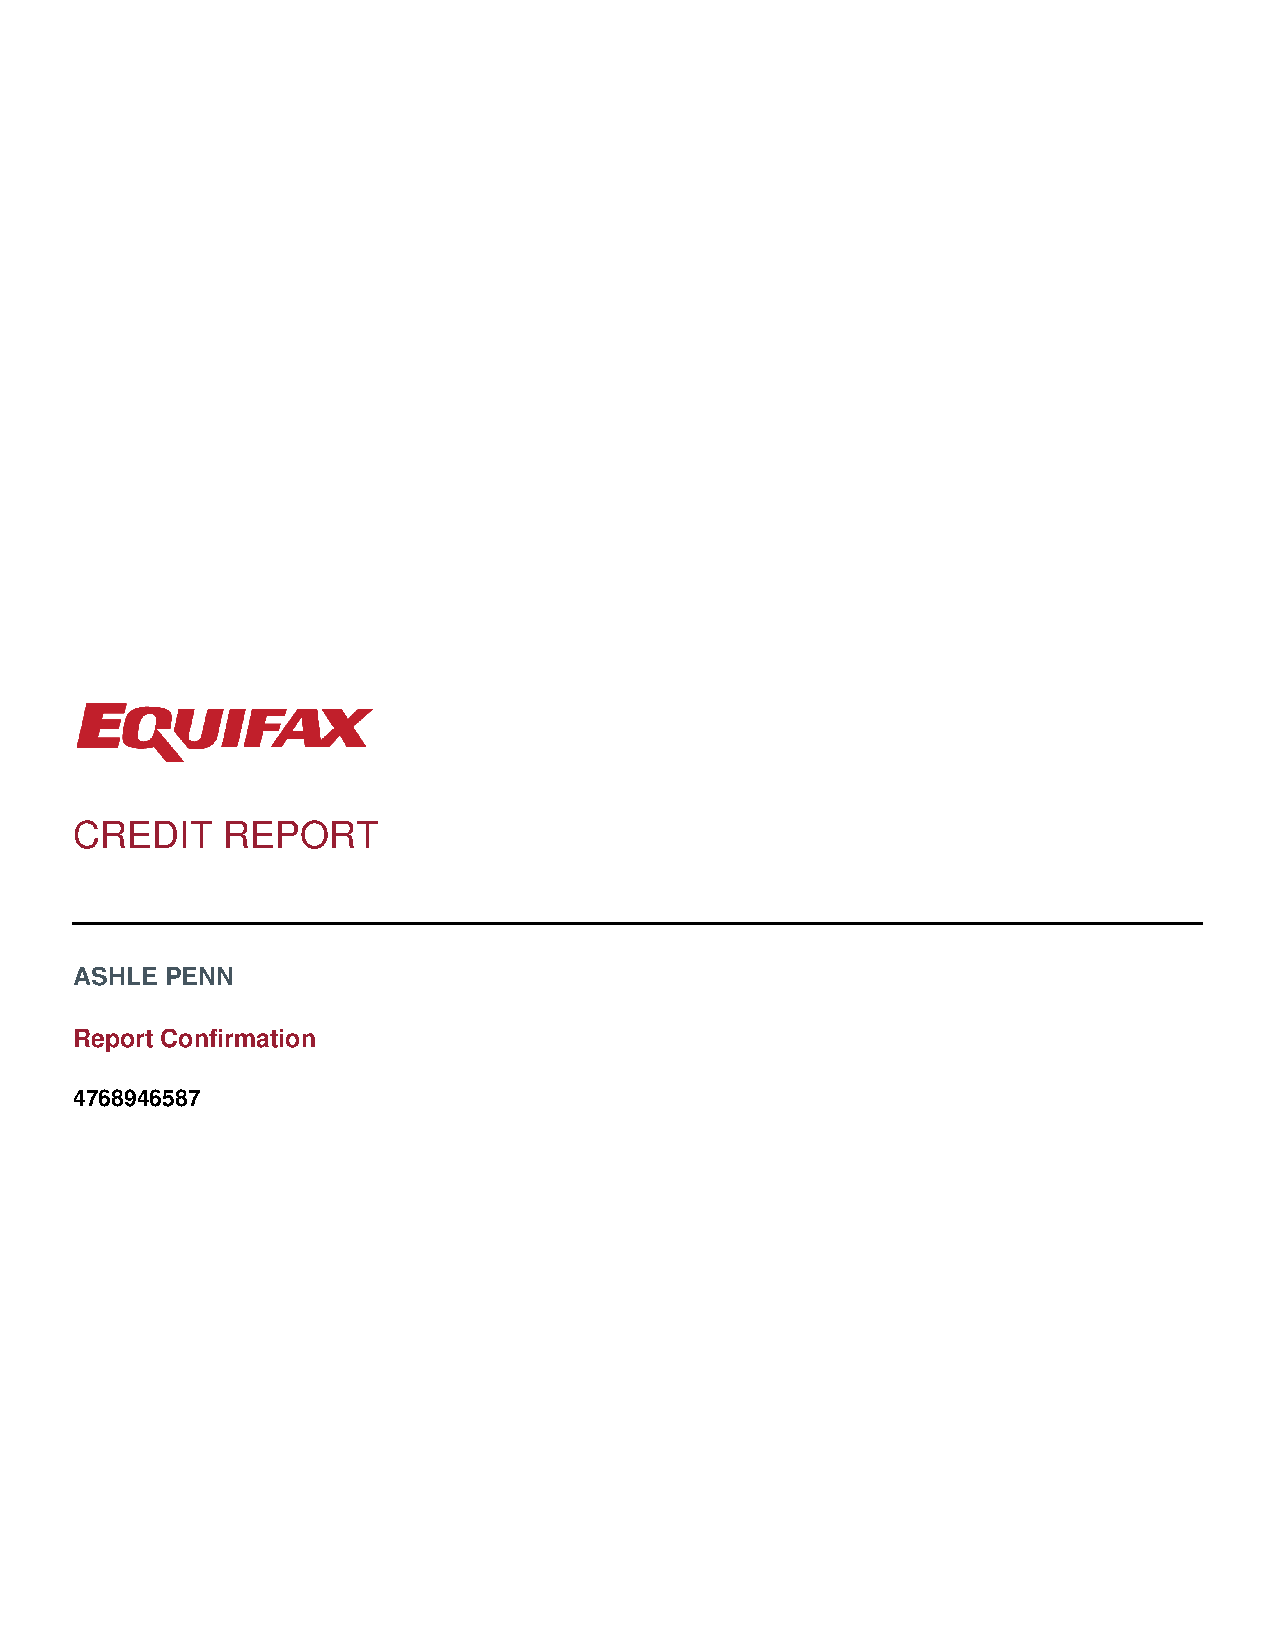
\includepdf[pages=-]{EQUIFAX_9.24.24.pdf}
\newpage \includepdf[pages=-]{EQUIFAX_3.1.26.pdf}
\newpage \includepdf[pages=-]{MPN.pdf}
\newpage \includepdf[pages=-]{TransUnion Credit Report.pdf}
\end{document}
